\documentclass{article}
\usepackage[margin=2cm]{geometry}
\usepackage{tabularx}
\usepackage{booktabs}
\usepackage{multirow}
\usepackage{enumitem}
\usepackage{url}
\usepackage{graphicx}
\usepackage{caption}
\usepackage{wrapfig}
\usepackage{setspace}
\usepackage{xcolor}
\usepackage{amsmath}
\usepackage{svg}



\makeatletter
\renewcommand{\maketitle}{\bgroup\setlength{\parindent}{0pt}
\begin{center} % Center the title
  \Large\@title
  \newline
  \footnotesize\@author
\end{center}
\begin{flushright}
  \@date
\end{flushright}
\egroup}
\makeatother

% Adjust line spacing
\setstretch{0.9}

% Adjust paragraph spacing
\setlength{\parskip}{0pt}

\begin{document}
\title{Impact of Liquidity Pool Size on Trading Volume in BTC-ETH Pools}
\author{
  Team \#111 \\
   \scriptsize Matias Vizcaino (avizcaino3) | Walter Jack Simmons (wsimmons35) | MingShen Wang (mwang709) | Vítor de Matos Castilho (vcastilho3)
}
\date{09 July 2023}
\maketitle



\noindent
{\setlength{\tabcolsep}{4pt} % Reduce column spacing

\section*{\textbf{Problem Statement and Objective}}

Decentralized Finance (DeFi), with a total value locked of approximately 48.78 billion USD (as of April 23, 2023 defillama.com), greatly depends on liquidity pools for efficient crypto trading. Liquidity pools, used in decentralized exchanges like Uniswap, function on an automated market maker model, unlike traditional exchanges that rely on intermediaries and order book systems. These pools generate income by collecting trading fees, which are subsequently distributed among liquidity providers based on their pool share.

Different platforms in the DeFi space, such as Curve Finance and Balancer, specialize in various areas, with Uniswap being a popular choice due to its user-friendly interface and diverse token pairs. 

The primary aim of this study is to \textbf{explore the impact of pool size on the trading volume, particularly focusing on BTC-ETH liquidity pools in decentralized exchanges like Uniswap}. We hypothesize a significant correlation between pool size and trading volume. Larger pools can theoretically support larger transactions and higher trading volumes due to the minimal price impact on large pools. This hypothesis is supported by DeFi: Modeling and Forecasting Trading Volume on Uniswap v3 Liquidity Pools2. 

Understanding this relationship can help optimize liquidity provision strategies, improve the efficiency of DeFi markets, and benefit various stakeholders. For instance, liquidity providers can increase fee returns and mitigate risks, while traders can enhance their strategies and reduce slippage. Our findings could also aid DeFi platforms in creating more effective liquidity pools to boost user engagement and overall growth.

\section*{\textbf{Introduction to Uniswap Liquidity Pools}}

In the decentralized finance (DeFi) space, there are various platforms that cater to different needs and focus on specific functionalities. Uniswap stands out as a popular choice among users. It is known for its user-friendly interface and wide range of token pairs available for trading. Other options are Curve Finance (for stablecoin and low-slippage trades) and Balancer (customizable pools with multiple tokens).

Uniswap is a decentralized exchange (DEX) on Ethereum that enables the trading of Ethereum-native and non-native assets (via wrapped coins like WBTC). Uniswap v3 utilizes a Constant Product Market Maker (CPMM) model where liquidity providers (LPs) deposit two tokens, maintaining a constant product of reserves. The prices are dynamically adjusted with trades, ensuring supply-demand balance.

The CPMM formula and liquidity pool price in terms of Token Y are given by:

\[x \cdot y = k \quad \text{and} \quad price = \frac{y}{x}\]

Here, \(x\) represents the quantity of Token X in the pool, \(y\) represents the quantity of Token Y in the pool, and \(k\) represents the constant product of the token reserves.

DEXs, like Uniswap, operate without a central authority, providing privacy, control over funds, and access to a wide range of tokens. However, centralized exchanges (CEX) offer faster transaction speeds, better user interfaces, customer support, and often higher liquidity. Despite this, CEXs hold user funds, exposing them to security risks.

Liquidity pools, mainly used in DEXs, allow traders to interact with smart contracts instead of other traders directly. This ensures constant liquidity availability but exposes LPs to risks such as impermanent loss. However, LPs receive transaction fee rewards proportional to their share in the pool.


Factors that influence prices include trade sizes, market conditions, token supply-demand dynamics, and external price changes.

Swaps involve exchanging one token for another in a liquidity pool. Swaps impact token prices as they modify the pool's token balances. Large swaps can cause significant price changes due to the constant product formula, leading to price slippage. Moreover, swap operations consume liquidity, affecting the overall pool liquidity.

Liquidity provision events, such as mints and burns, have a notable impact on trading volumes. Minting tokens increases liquidity, attracting more traders and potentially boosting trading volume. Conversely, burning tokens reduces liquidity and may result in decreased trading volume.

While liquidity events in one pool do not directly affect others, indirect effects arising from network correlations and arbitrage opportunities can influence trading volumes across multiple pools. For instance, a substantial increase in liquidity in one pool can attract more traders across the network, indirectly affecting trading volumes in other pools.

\section*{Dataset}

Inspired by the \textit{"DeFi modeling and forecasting trading volume" (2023)}\footnote{\textit{"DeFi: modeling and forecasting trading volume on Uniswap v3 liquidity pools"} (2023), \url{https://ssrn.com/abstract=444535}.} paper, we sourced and constructed trade information for at least 6 months. Initial extraction work has already been performed, and you can refer to our GitHub repository\footnote{GitHub repository: \url{https://github.gatech.edu/MGT-6203-Summer-2023-Canvas/Team-111/tree/main/Code}} for further details and access to the code. The dataset consists of data obtained from the following sources:


\begin{center}
\begin{tabular}{|p{0.15\linewidth}|p{0.35\linewidth}|p{0.5\linewidth}|}
\hline
\textbf{Source} & \textbf{Description} & \textbf{Data} \\
\hline
Uniswap's The Graph API\footnote{Uniswap's The Graph API: \url{https://api.thegraph.com/subgraphs/name/uniswap/uniswap-v3}} & Provides transaction details, trading volumes, and block information from Uniswap v3 liquidity pools. & Transaction IDs, timestamps, amounts, USD equivalents, and other related data. \\
\hline
Etherscan API\footnote{Etherscan API: \url{https://api.etherscan.io/api}} for Uniswap transaction hashes & Used to extract corresponding transaction data from Etherscan based on transaction hashes. & Block hashes, block numbers, sender addresses, gas details, transaction hashes, and other relevant information. \\
\hline
Binance\footnote{Binance GitHub Repository: \url{https://github.com/binance/binance-public-data/blob/master/python/README.md}} CEX Data for ETHBTC & Daily zip trades downloaded using provided scripts from the Binance GitHub repository. & Detailed information about each trade executed on the Binance platform, including trade prices, quantities, timestamps, and buyer/seller characteristics. \\
\hline
\end{tabular}
\end{center}


\section*{Key Variables}
\textbf{Target Variable:} Liquidity pool trading volumes (amountUSD) over specific blocks. We consider different models for multiple time horizons to study the relationship change over time.

\textbf{Independent Variables:}
The dependent variables are derived from a set of features and are categorized as follows:
\begin{enumerate}[label=\arabic*. ,itemsep=0pt, topsep=0pt]
\item Direct pool features (43): volatility, rate, number of trades, average trade size, total value locked (TVL). [Mostly completed, refer to progress section]
\item Network spillover effects (8): trade flow imbalance. [Not yet started]
\item CEX spillover effects (6): actual coin trade volume. [Not yet started]
\item Price divergences between the 500 and 3000 pools (2). [Not yet started]
\end{enumerate}
We will aim to include as many variables as possible, given the time constraints of our project.

\section*{Approach and Progress}
\section*{Progress Report}

\begin{table}[htbp]
\centering
\small
\begin{tabularx}{\linewidth}{|>{\raggedright\arraybackslash}X|}
\hline
\textbf{Data Collection:} Sourced data from multiple APIs (Uniswap, Binance) for liquidity pool sizes, trading volumes, and relevant variables. Data has been associated with Ethereum block numbers for consistent time measurement. Despite API rate limits, most of the data has been collected successfully. \\
\hline
\textbf{Data Preprocessing:} Cleaned, formatted, and addressed missing values in the dataset. Data consistency ensured and discrepancies from multiple sources addressed. Preprocessing completed with further examination of missing values in independent variables. Records with null values temporarily removed for continued analysis. \\
\hline
\textbf{Feature Engineering:} Constructed features to capture historical patterns, spillover effects, and price divergences utilizing a block-based time-series analysis framework. Feature engineering mostly complete, handling most direct pool features with finite lag. A review is planned to reduce the number of null values, include other feature categories, and perform feature selection. \\
\hline
\textbf{Exploratory Data Analysis:} Generated descriptive statistics, visualizations, and performed correlation analyses to uncover patterns, trends, and relationships between variables. In-depth exploratory data analysis will be performed once all features have been engineered, with various correlations and trends identified among the variables. \\
\hline
\textbf{Model Selection and Development:} Implemented a multivariate regression model (OLS) to investigate the pool size-trading volume relationship. Predicted target variables at different horizons with the application of lagged variables. OLS regression models have been developed and tested. Additional model testing and optimization in progress. \\
\hline
\textbf{Model Evaluation and Optimization:} Models evaluated using R-squared metric. Initial analyses indicate that model performance can be enhanced through further feature engineering/selection and reducing multicollinearity. Conducting correlation analysis and Variance Inflation Factor (VIF) for the final features. \\
\hline
\textbf{Final Analysis and Conclusions:} In the final stages of analysis. Commencing with drawing conclusions and communicating findings. Preparing to provide quantitative-driven insights. \\
\hline
\end{tabularx}
\end{table}




Overall, significant progress has been made in each stage of our approach. However, further analysis, evaluation, and optimization are required to successfully complete the project.

Throughout this process, we aim to maintain rigorous documentation of our methodologies and findings, which will allow us to ensure the transparency and replicability of our research.

\section*{Challenges and Insights}

The engineering required to collect, merge and generate features has been more advanced than initially expected, and so considerable time and effort has been placed in this regard.
In terms of data collection, API calls are built on Python (and circumvent request limitations) to gather the necessary data in JSON formats. Particularly challenging has been the Etherscan free-tier API rate limits, which takes several days to extract 6 months of transaction data. We are still running downloads, so our dataset remains incomplete, in particular for transactions on pool 3000.

\begin{wrapfigure}[19]{r}{0.35\textwidth}
\vspace{-35pt} % Adjust the vertical spacing as needed
\centering
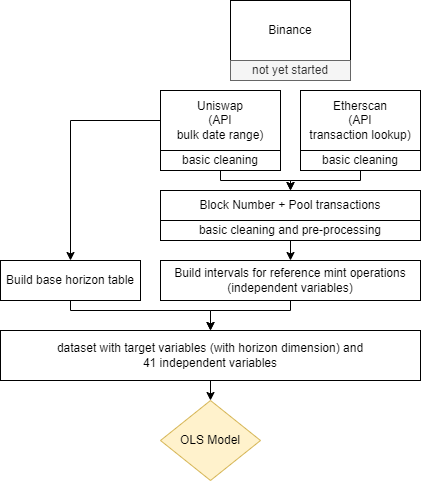
\includegraphics[width=\linewidth]{C:/Users/MatiasVizcaino/repos/6203-DataAnalyticsBusiness-Project/Other Resources/data-diagram.drawio.png}
\caption{Data Engineering}
\label{fig:data-diagram}
\end{wrapfigure}

Particularly interesting to tackle but also complex and time-consuming has been to deal with two different concepts of time being used:
First, the "trading clock" is defined by a block where a mint operation occurs (i.e., This is used to define a finite lag effect in the independent variables, capturing the temporal dynamics of the data or delay effects for events that change liquidity and pricing of pools).
Secondly, a time horizon concept is formed that consists of every ten blocks, up to the next mint operation. This is used to study a temporal element in the target variable, facilitating a deeper understanding of the liquidity pool dynamics and helps identify patterns, trends, or variations in the predictive power of the independent variables for different horizons. 

Combined, the time series enables the exploration of short-term variations and long-term trends, enhancing the accuracy and depth of the analysis.  It provides valuable insights for decision-making, strategy optimization, and risk management in the decentralized finance ecosystem.
It is important to note that in Ethereum, every block takes around 14 seconds and Uniswap operates on the Ethereum blockchain.

The mathematics of liquidity pools have also proven to be a barrier-to-entry into this type of analysis. We aim to encapsulate the formulas to the best of our understanding in the calculations.py functions. Given more time, we would probably further explore and optimise the calculations for deriving more features.

\section*{Progress}

\subsection*{Engineering}

The primary focus has been on the design of the Target Variable and the determination of its temporal horizons. Concurrently, we have tackled the challenging task of feature engineering for the Direct pool features with finite lag. Despite the complexity, we remain confident in our ability to meet the remaining objectives within the established timeline. 

In terms of merging Uniswap transactions with Etherscan, we've observed a high match rate of transactions for the analysis period of six months. The transaction breakdown is as follows:

Total uniswap transactions:
[((500, 'burns'), 4000), ((500, 'mints'), 3406), ((500, 'swaps'), 217821), ((3000, 'burns'), 5918), ((3000, 'mints'), 5046), ((3000, 'swaps'), 48592)]
Total uniswap<>etherscan transactions:
[((500, 'burns'), 4000), ((500, 'mints'), 3242), ((500, 'swaps'), 217821), ((3000, 'burns'), 5918), ((3000, 'mints'), 4986), ((3000, 'swaps'), 48592)]

From the transaction data, we created 8,227 reference blocks that correspond to each mint operation, excluding one. These blocks were then used to engineer features to calculate metrics for the same pool and other pools. These features capture data about liquidity pools and calculate metrics such as volatility, traded volume rate, trades count, and average volume. To expand the analysis, we have also included lagged features for the previous three mint operations. The table below serves as our block reference table:

\begin{table}[htbp]
  \centering
  \small
  \begin{tabularx}{\linewidth}{|X|r|l|l|}
    \hline
    \textbf{pool} & \textbf{blockNumber} & \textbf{blockNumberChain} & \textbf{other\_blockNumberChain} \\
    \hline
    500 & 14498564 & [14498564, nan, nan, nan] & [14498564, nan, nan, nan] \\
    500 & 14498699 & [14498699, 14498564, nan, nan] & [14498699, nan, nan, nan] \\
    500 & 14499597 & [14499597, 14498699, 14498564, nan] & [14499597, 14499560, 14499457, 14499198] \\
    500 & 14499836 & [14499836, 14499597, 14498699, 14498564] & [14499836, 14499560, 14499457, 14499198] \\
    500 & 14500355 & [14500355, 14499836, 14499597, 14498699] & [14500355, 14500043, 14499560, 14499457] \\
    ... & ... & ... & ... \\
    3000 & 15648981 & [15648981, 15648330, 15648305, 15648187] & [15648981, 15648887, 15648536, 15646933] \\
    3000 & 15649246 & [15649246, 15648981, 15648330, 15648305] & [15649246, 15649243, 15648887, 15648536] \\
    3000 & 15649545 & [15649545, 15649246, 15648981, 15648330] & [15649545, 15649522, 15649347, 15649269] \\
    3000 & 15649565 & [15649565, 15649545, 15649246, 15648981] & [15649565, 15649522, 15649347, 15649269] \\
    3000 & 15649578 & [15649578, 15649565, 15649545, 15649246] & [15649578, 15649522, 15649347, 15649269] \\
    \hline
  \end{tabularx}
  \caption{Your table caption}
  \label{tab:my-table1}
\end{table}

Before initiating the modeling phase, we need to address records with missing values in the independent variables. Notably, some null values have been identified in the volatility (same pool) and avg-USD/rate-USD (other pool) metrics. We have opted to remove these records temporarily to proceed with the analysis, with plans to reassess the calculations and mitigate the occurrence of null values likely resulting from lagged variables.

Finally, we've constructed a base table with the \texttt{start\_blockNumber} of each horizon and the \texttt{reference\_blockNumber}, defined by mint operations in the block. This base table is joined with the mint aggregated transaction data to generate our target variables and independent variables that are lagged.

\vspace{2em} % Add some vertical spacing
\begin{table}[htbp]
  \centering
  \small
  \begin{tabular}{cccccc}
    \hline
    \textbf{blockNumber} & \textbf{min\_flag} & \textbf{reference\_blockNumber} & \textbf{horizon\_label} & \textbf{cum\_volume\_500} \\
    \hline
    108757 & 0 & 15552674 & 9 & 423485.346309 \\
    108758 & 0 & 15552674 & 10 & 423485.346309 \\
    108759 & 1 & 15552772 & 1 & 328338.732259 \\
    108760 & 0 & 15552772 & 2 & 406084.780730 \\
    108761 & 0 & 15552772 & 3 & 536640.714920 \\
    ... & ... & ... & ... & ... \\
    109047 & 0 & 15555464 & 12 & 122730.731534 \\
    109048 & 0 & 15555464 & 13 & 123650.594764 \\
    109049 & 0 & 15555464 & 14 & 123650.594764 \\
    109050 & 1 & 15555597 & 1 & 104.152423 \\
    109051 & 0 & 15555597 & 2 & 971.612926 \\
    \hline
  \end{tabular}
  \caption{Your table caption}
  \label{tab:my-table}
\end{table}

\subsection*{Modelling}

We have commenced the development of a framework for our prediction models and have constructed several Proof of Concept (PoC) models. For the modeling phase, we're employing an Ordinary Least Squares (OLS) regression approach to predict multiple target variables across different horizons using a set of independent lagged variables for each reference mint. This process involves iterating over the horizons, generating data subsets, fitting an OLS model for each horizon, and retrieving the R-squared value as a performance indicator. This approach allows for efficient and consistent prediction across various horizons.

\[
\text{{cum\_volume\_500}}_\text{{horizon}} = \beta_0 + \beta_1 \cdot \widetilde{01}X + \beta_2 \cdot \widetilde{12}X + \beta_3 \cdot \widetilde{23}X + \ldots + \epsilon
\]

In this formula, \(\beta_0\), \(\beta_1\), \(\beta_2\), \(\beta_3\), etc., represent the coefficients associated with each spot lagged variable, while \(\epsilon\) denotes the error term or residual.

\begin{wrapfigure}[12]{l}{0.35\textwidth}
\vspace{-15pt} % Adjust the vertical spacing as needed
\centering
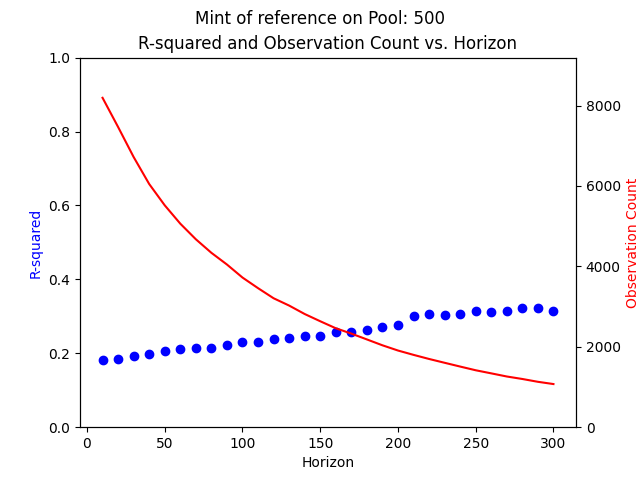
\includegraphics[width=\linewidth]{C:/Users/MatiasVizcaino/repos/6203-DataAnalyticsBusiness-Project/Other Resources/R2Horizon.png}
\caption{R2 best fit horizon}
\label{fig:R2-horizon}
\end{wrapfigure}

Observations indicate that around the horizon 20 (200 blocks, approximately 13 minutes), the R2 value ceases to increase significantly. Preliminary analysis of the relevant model (at horizon 20) reveals that the OLS regression model explains approximately 27.6\% of the variation in the dependent variable cum\_volume\_3000\_ref500. The significant variables, such as rate-count-isame\_01, rate-count-isame\_12, rate-count-isame\_23, and wlother\_3, have a considerable impact on the dependent variable. However, the potential collinearity among the independent variables could affect the interpretation of individual coefficients, suggesting a need for further analysis.

Model selection will be based on the optimal combination of features for each horizon. As we refine the feature and model development, considerations like autocorrelation, endogeneity, structural breaks, or multicollinearity will be addressed. These will be managed through additional sensitivity analyses, cross-validations, and the application of appropriate statistical techniques to diagnose and mitigate any complexities.

\section*{Going Forward}

Given the extensive nature of the data engineering activities involved in this project, we anticipate that these activities will continue throughout further feature engineering and feature selection processes.
Similarly, our next steps in the modeling phase include:

\begin{itemize}
    \item Dataset Splitting: We will divide the dataset into training and test sets and conduct model metrics analysis and interpretations.
    \item Analysis Scope: We will perform analysis on both Pool 500 and Pool 3000, specifically focusing on target variables related to volume on the same pool as the reference mint, the other pool, or both.
    \item Experimentation: We will carry out experiments to identify the best combinations of features, horizons, and target variables that yield the most accurate predictions.
    \item Feature selection: By using techniques such as step-wise or Principal Component Analysis, reduce the number of features to make the model less complex, reduce overfitting, and more interpretable.
\end{itemize}

Some possible experiments we plan to conduct include trying different lag lengths, incorporating quadratic features and/or interaction terms, and accounting for structural breaks such as the Terra-Luna collapse in May 2022 and the Merge in September 2022.

We aspire that a complete analysis allows us to provide quantitative-driven discussion on:
\begin{enumerate}[itemsep=0pt, topsep=0pt]
\item What is the relationship between liquidity pool size and trading volume in BTC-ETH liquidity pools?
\item How does the size of the liquidity pool influence the slippage in BTC-ETH trading pairs? (i.e., by analysing CEX spillover effects)
\item How does BTC-ETH price volatility affect trading volume relative to liquidity pool size? (i.e., by analysing price divergence)
\item Are there specific periods or events that significantly influence the relationship between the size of the BTC-ETH liquidity pool and its trading volume?
\end{enumerate}


\end{document}